%%
%% 2019 07 04 Ph. G. Freimann
%%

\section{Rechtwinkliges Dreieck}\index{Dreieck!rechtwinkliges}\index{rechtwinkliges Dreieck}
\sectuntertitel{... nein, wir sind nicht Asterix und Obelix: Wir sind
  Römer, wir sind Sinus und Cosinus ...\footnote{S. Asterix -- Tour de France -- Seite 40}}

\theorieTALSGeom{84}{2.1}
%%\theorieGESO ????
%%%%%%%%%%%%%%%%%%%%%%%%%%%%%%%%%%%%%%%%%%%%%%%%%%%%%%%%%%%%%%%%%%%%%%%%%%%%%%%%%
\subsection*{Lernziele}

\begin{itemize}
 \item Satz des Pythagoras Formel
 \item Höhensatz
 \item sinus/cosinus/tangens
\end{itemize}



%% include Allgemeine Form und Höhensatz
%% Einbinden in Trigo: Rechtwinkliges Dreieck, aber auch
%% in Planimetrie: Satz des Pythagoras
%%
%% Hier:
%%   * Allgemeine Form
%%   * Höhensatz
%%   Nicht dabei:
%5     -Sinus/Cosinus/Tangens (dies ist nur in Trigo)
%5     -Höhensatz (der kommt nur bei der Planimetrie)



%% Load this only once (the first occurence)!
%% see here: https://tex.stackexchange.com/questions/195157/is-there-any-analog-to-pragma-once-in-latex
\ifcsname XX_Pythagoras.tex\endcsname
  \expandafter\endinput
\fi
\expandafter\gdef\csname XX_Pythagoras.tex\endcsname{loaded}



%%%%%%%%%%%%%%%%%%%%%%%%%%%%%%%%%%%%%%%%%%%%%%%%%%
\newpage

\subsection{Rechtwinkliges Dreieck}

\definecolor{qqwuqq}{rgb}{0,0.39,0}
\definecolor{xdxdff}{rgb}{0.49,0.49,1}
\definecolor{qqqqff}{rgb}{0,0,1}
\begin{tikzpicture}[line cap=round,line join=round,>=triangle 45,x=1.0cm,y=1.0cm]
\clip(-0.54,0.17) rectangle (5.83,4.51);
\draw [shift={(3.35,3.58)},color=qqwuqq,fill=qqwuqq,fill opacity=0.1] (0,0) -- (-154.75:0.95) arc (-154.75:-64.75:0.95) -- cycle;
\draw (0,2)-- (4.56,1.02);
\draw (0,2)-- (3.35,3.58);
\draw (3.35,3.58)-- (4.56,1.02);
\fill[color=qqwuqq,fill=qqwuqq,fill opacity=0.1] (3.16,3.05) circle (0.03);
\begin{scriptsize}
\fill [color=qqqqff] (0,2) circle (1.5pt);
\draw[color=qqqqff] (0.25,2.42) node {$A$};
\fill [color=qqqqff] (4.56,1.02) circle (1.5pt);
\draw[color=qqqqff] (4.81,1.44) node {$B$};
\fill [color=xdxdff] (3.35,3.58) circle (1.5pt);
\draw[color=xdxdff] (3.61,4.01) node {$C$};
\draw[color=qqwuqq] (2.37,2.49) node {$90\textrm{\degre}$};
\end{scriptsize}
\end{tikzpicture}

\begin{definition}{Rechtwinkliges Dreieck}{}
Im \textbf{rechtwinkligen} Dreieck misst der Winkel gegenüber der
längsten Seite 90\degre.
\end{definition}



\subsection{Satz des Pythagoras (Repetition)}\index{Pythagoras!Satz des|textbf}\index{Satz des Pythagoras|textbf}

\begin{gesetz}{Satz des Pythagoras}{}
Im rechtwinkligen Dreieck mit Hypotenuse $c$ gilt:
$$a^2 + b^2 = c^2$$
\end{gesetz}

\TNTeop{Platz für graphischen Beweis\vspace{3cm}}



%%%%%%%%%%%%%%%%%%%%%%%%%%%%%%%%%%%%%%%%%%%%55
\subsection{Höhensatz}\index{Höhensatz}

Im rechtwinkligen Dreieck gilt:
$$h^2=p\cdot{}q$$

Beweise:

\TNT{6.4}{

Beweis mit Ähnlichkeit: $p:h = h:q$, somit folgt der Satz direkt.

Optional: Beweis mit Pythagoras: $h^2 = a^2 - p^2$ und $h^2 = b^2 -
  q^2$.\\
Somit gilt
$2h^2 = a^2 + b^2 - p^2 - q^2 = c^2 - p^2 - q^2 = (p+q)^2 -p^2 - q^2 =
  p^2 +2pq + q^2 - p^2 - q^2 = 2pq$\\
Daraus folgt:$$h^2=pq.$$
}

\subsection*{Aufgaben}
\AadBMTG{37}{8., 9., 15., }

\newpage

\subsection{Spezielle Dreiecke}\index{Dreiecke!spezielle}

\subsubsection*{Lernziele}
\begin{itemize}
  \item 45\degre: Das halbe Quadrat\index{Quadrat}
  \item 30\degre/60\degre: Das halbe gleichseitige
  Dreieck\index{Dreieck!gleichseitiges}\index{gleichseitiges Dreieck}
\end{itemize}

\TadBMTG{33}{2.4.1}



\begin{samepage}
\subsection{gleichseitiges Dreieck und halbes Quadrat}\index{Dreieck!gleichseitiges}\index{gleichseitiges Dreieck}\index{Quadrat!Diagonale}\index{halbes Quadrat}

\renewcommand{\arraystretch}{2.4}
\begin{tabular}{|c|p{5cm}|} 
  \hline
  \raisebox{-18mm}{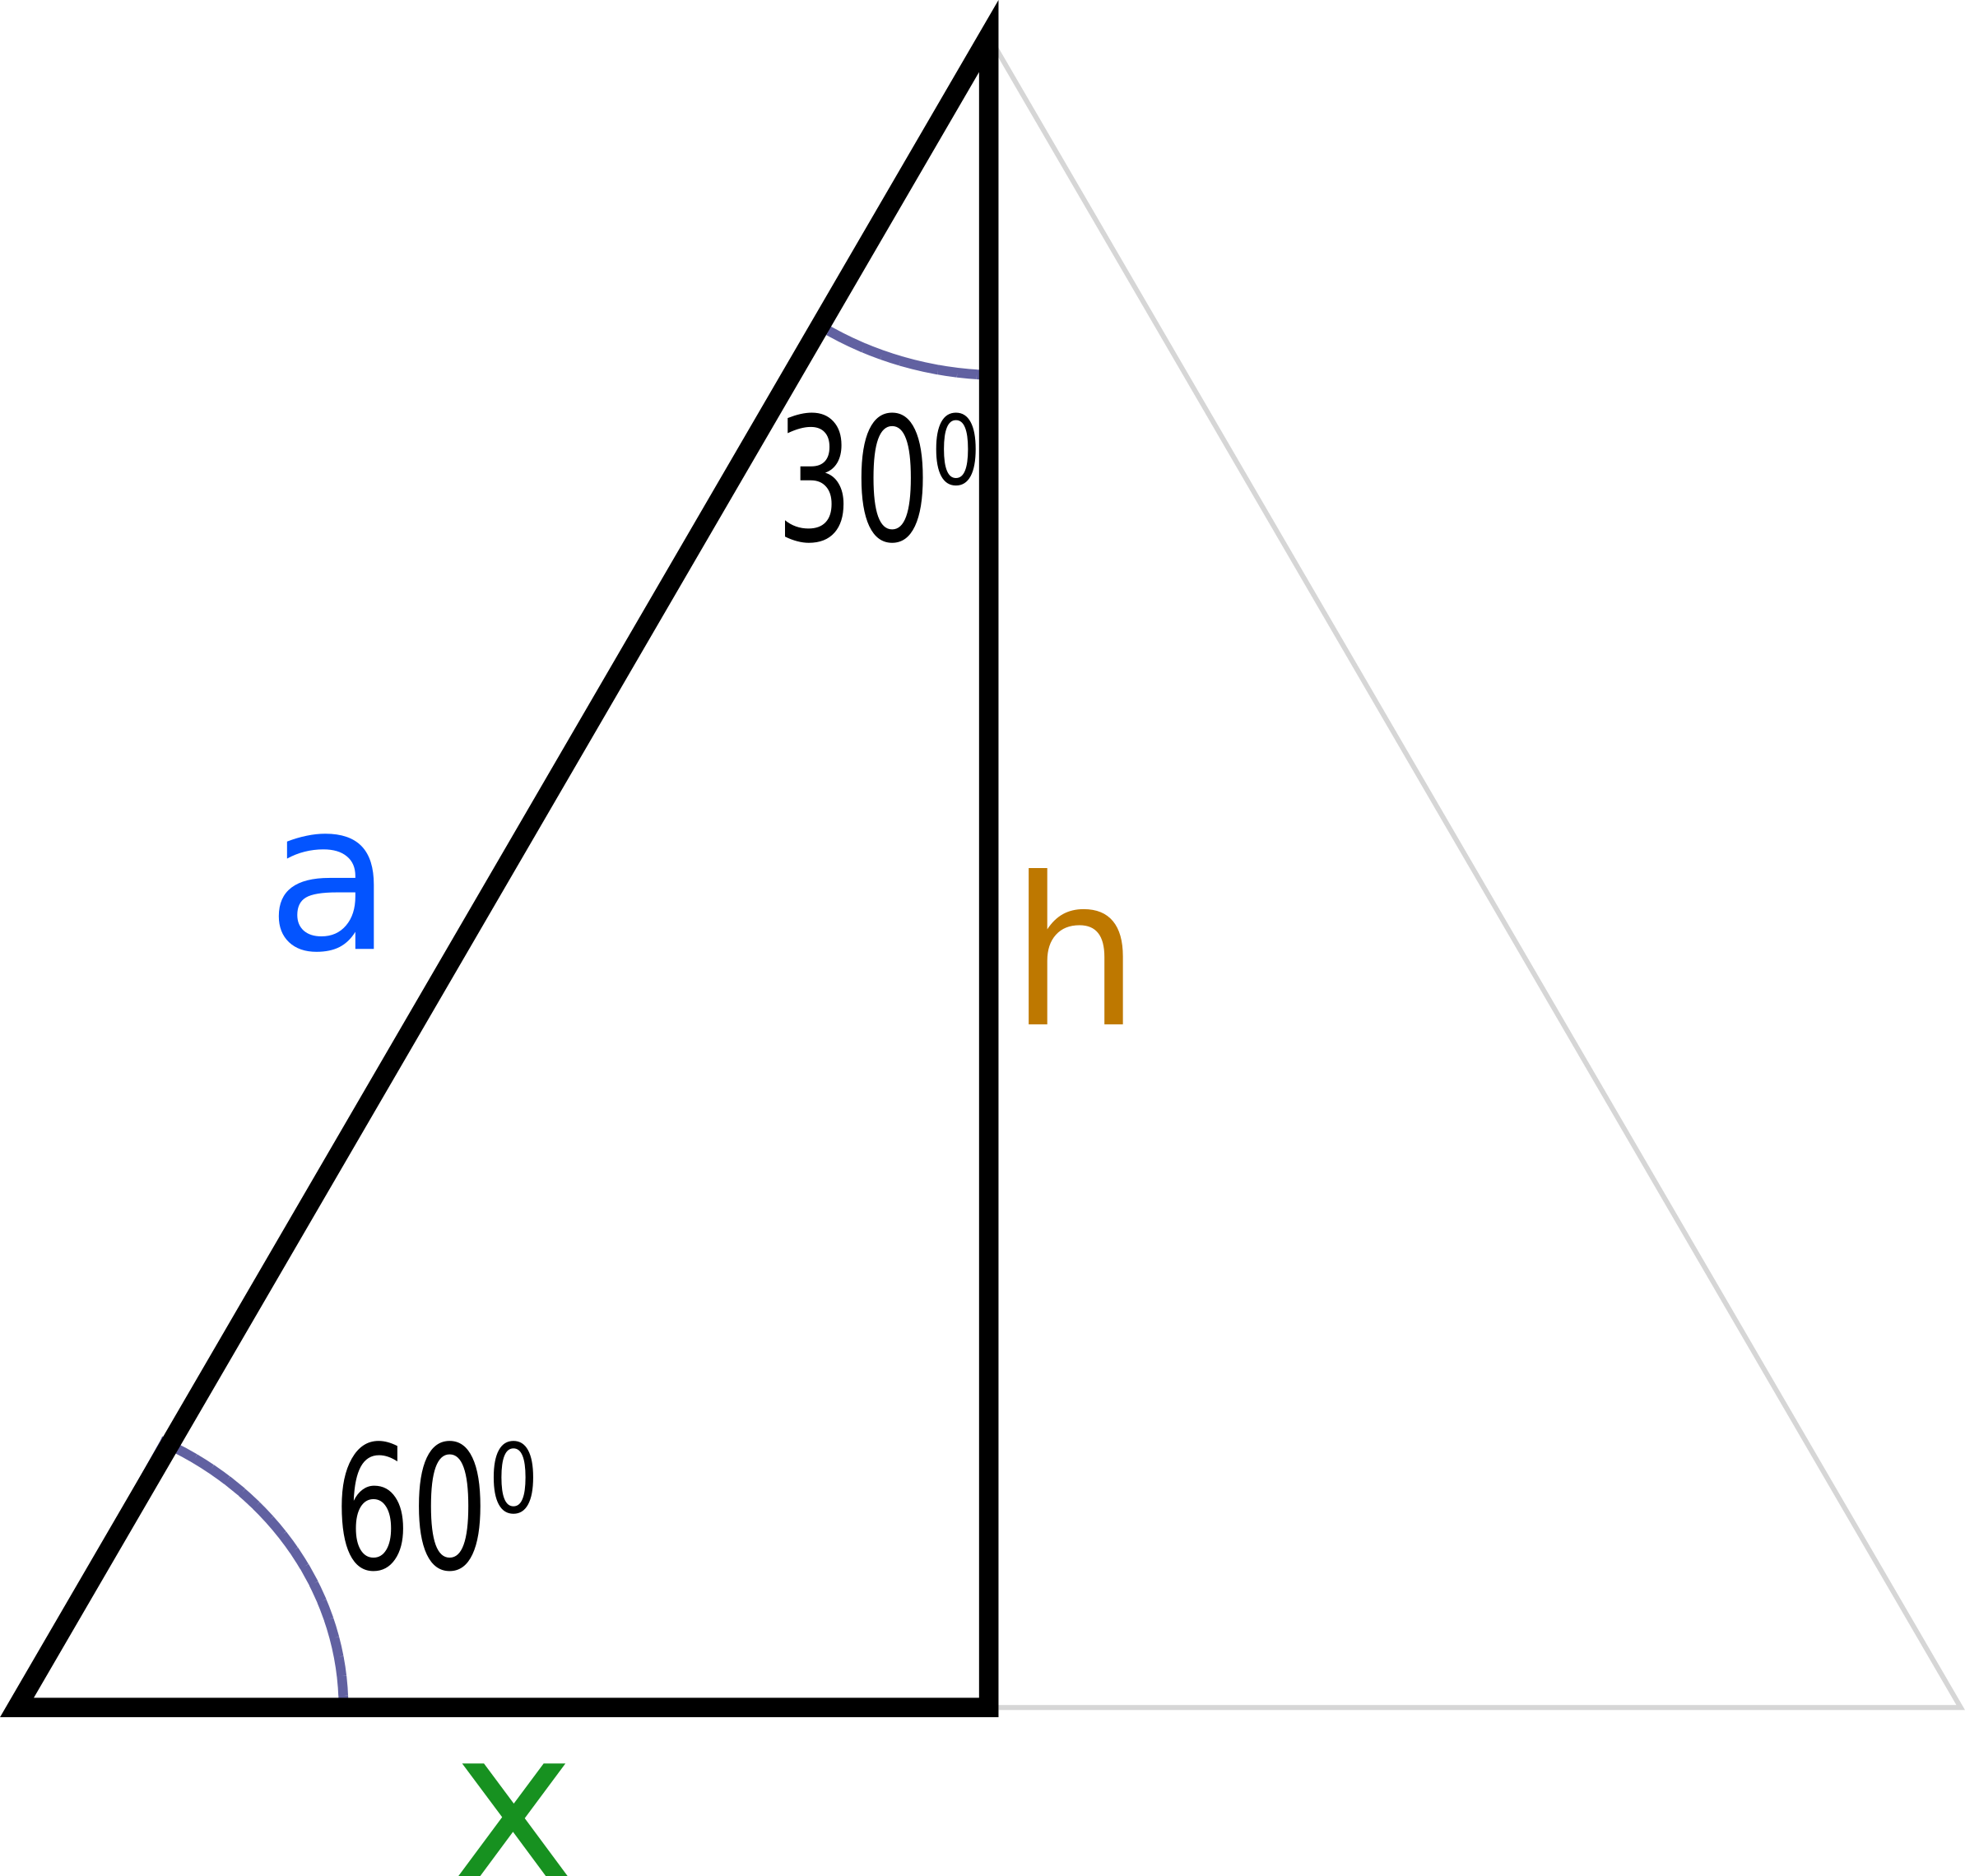
\includegraphics[width=4cm]{tals/plani/img/gleichseitigesDreieck.png}} &
  $\begin{array}{ll}
    x=& \frac{a}{2}                     \\
    h=& \sqrt{3}\cdot{}x                \\
    h=& \frac{\sqrt{3}}{2}\cdot{}a
  \end{array}$ \\

  \hline
  \raisebox{-24mm}{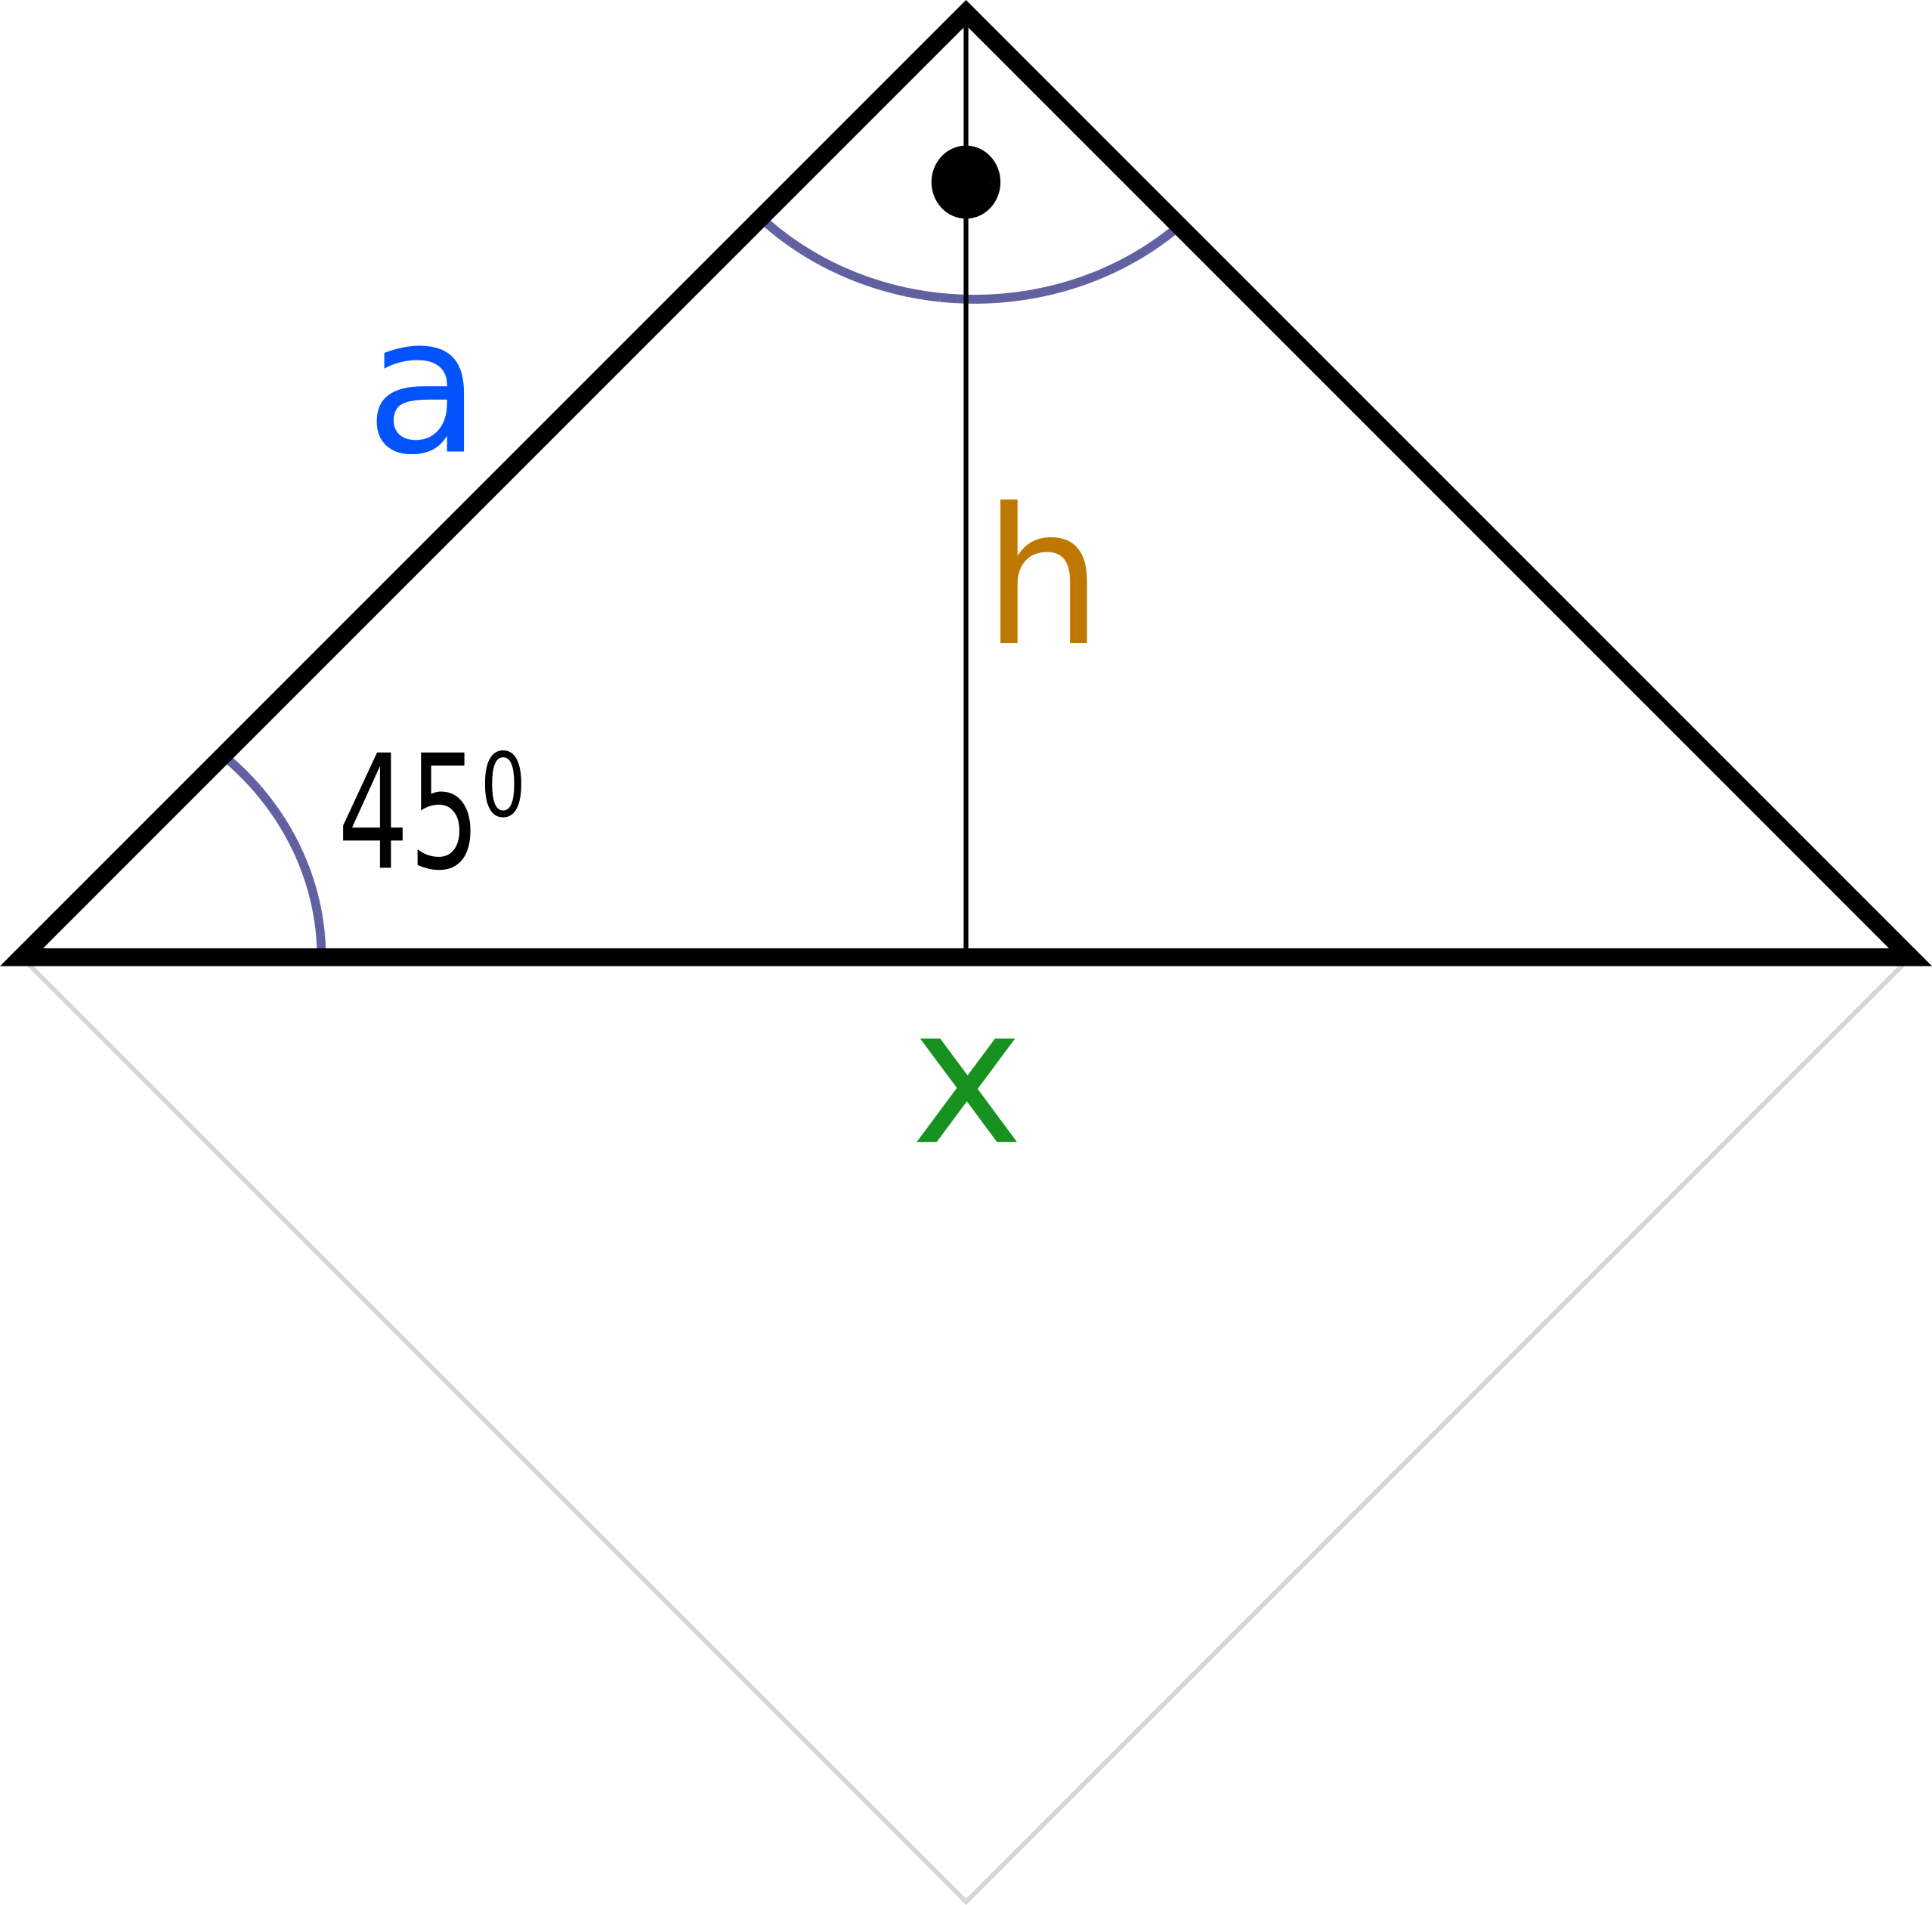
\includegraphics[width=5cm]{tals/plani/img/halbesQuadrat.png}} &
  $\begin{array}{ll}
    x=& \sqrt{2}\cdot{}a            \\
    h=& \frac{x}{2}                 \\
    h=& \frac{\sqrt{2}}{2} \cdot{} a\\
    a=& \sqrt{2}\cdot{}h
  \end{array}$ 
  \\
  
  \hline
\end{tabular} 
\renewcommand{\arraystretch}{1}

\TALS{Siehe auch \cite{frommenwiler18geom} S. 25 Kapitel 1.2.2}

\end{samepage}



\subsection*{Aufgaben}
\AadBMTG{37}{7., 11., 12., 13., 19., 20., 21., 24., 26., 27., 28.,
29., 30., 33., 34., 40. und 41. }
\newpage



\subsection{Rechtwinkliges Dreieck}

\definecolor{qqwuqq}{rgb}{0,0.39,0}
\definecolor{xdxdff}{rgb}{0.49,0.49,1}
\definecolor{qqqqff}{rgb}{0,0,1}
\begin{tikzpicture}[line cap=round,line join=round,>=triangle 45,x=1.0cm,y=1.0cm]
\clip(-0.54,0.17) rectangle (5.83,4.51);
\draw [shift={(3.35,3.58)},color=qqwuqq,fill=qqwuqq,fill opacity=0.1] (0,0) -- (-154.75:0.95) arc (-154.75:-64.75:0.95) -- cycle;
\draw (0,2)-- (4.56,1.02);
\draw (0,2)-- (3.35,3.58);
\draw (3.35,3.58)-- (4.56,1.02);
\fill[color=qqwuqq,fill=qqwuqq,fill opacity=0.1] (3.16,3.05) circle (0.03);
\begin{scriptsize}
\fill [color=qqqqff] (0,2) circle (1.5pt);
\draw[color=qqqqff] (0.25,2.42) node {$A$};
\fill [color=qqqqff] (4.56,1.02) circle (1.5pt);
\draw[color=qqqqff] (4.81,1.44) node {$B$};
\fill [color=xdxdff] (3.35,3.58) circle (1.5pt);
\draw[color=xdxdff] (3.61,4.01) node {$C$};
\draw[color=qqwuqq] (2.37,2.49) node {$90\textrm{\degre}$};
\end{scriptsize}
\end{tikzpicture}


\subsection{$\sin{}$, $\cos{}$ und $\tan{}$}
\TALS{(Theorie S. 84 Kap. 2.1 \cite{frommenwiler18geom})}


\newpage
\subsection{Fläche im allgemeinen Dreieck}\index{Fl\"ache!Dreieck}
\TALS{(S. 96 Kap. 2.1.3 \cite{frommenwiler18geom})}

\bbwCenterGraphic{6cm}{tals/trig1/img/dreieck_sws.png}

Im allgemeinen Dreieck kann die Fläche A wie folgt berechnet werden:
$$A = \frac{1}{2}\cdot{}b\cdot{}c\cdot{}sin(\epsilon)$$
Also die Hälfte von Seite mal Seite mal Sinus des Zwischenwinkels.
\newpage


\subsection{Steigung vs. Winkel}\index{Steigung}

\bbwCenterGraphic{4.5cm}{tals/trig1/img/starkeSteigung.jpg}

Steigungen werden üblicherweise in \% angegeben. Das obige
Verkehrsschild «starke Steigung» gibt 10\% an. Das heißt:

\TNT{3.6}{Auf einen horizontalen Meter, steigt die Straße um 10cm (=
  10\%).
\vspace{3cm}}

Um den Winkel zu berechnen, kann der Tangens verwendet werden:
$$\frac{0.10m}{1.00m} = \tan(\sigma)$$
In obigem Beispiel ist der Steigungswinkel also durch den $\arctan()$
berechenbar:

$$\sigma = \arctan\left(\frac{0.1m}{1.0m}\right) = \arctan(0.1) \approx 5.71\degre$$
\newpage
%% Sinushand
\subsection{Merkregel der wichtigsten Sinus-Werte}\index{Sinushand}
\bbwCenterGraphic{12cm}{tals/trig1/img/sinushand.png}
Anstelle des Ablesens im Gleichseitigen Dreieck kann man sich die wichtigsten Werte
auch mit obiger ``Sinushand'' merken:

\TRAINER{%%
\begin{tabular}{r|l|c|l}
      & $sin()$                              & $\cos()$             & $\tan()=\frac{\sin()}{\cos()}$              \\\hline
   0  & $\frac{\sqrt{\textbf{0}}}{2} = 0$    & 1                    &   0                                         \\\hline
  30  & $\frac{\sqrt{\textbf{1}}}{2} = 0.5 $ & $\frac{\sqrt{3}}{2}$ &  $\frac{1}{\sqrt{3}} = \frac{\sqrt{3}}{3}$  \\\hline
  45  & $\frac{\sqrt{\textbf{2}}}{2}$        & $\frac{\sqrt{2}}{2}$ &   1                                         \\\hline
  60  & $\frac{\sqrt{\textbf{3}}}{2}$        & 0.5                  &  $\sqrt{3}$                                 \\\hline
  90  & $\frac{\sqrt{\textbf{4}}}{2} = 1$    & 0                    & nicht definiert
\end{tabular}
}%% END TRAINER

\noTRAINER{%%
\begin{tabular}{r|l|c|l}
      & $sin()$  & $\cos()$  &  $\tan()=\frac{\sin()}{\cos()}$        \\\hline
   0  &          &           &         \\\hline
  30  &          &           &         \\\hline
  45  &          &           &         \\\hline
  60  &          &           &         \\\hline
  90  &          &           &         \\
\end{tabular}
}%% END noTRANIER
\newpage

\subsection*{Aufgaben}
\TALSGeomAadB{84ff}{2. alle 3. a) b) e) 4. a) c) 6. a) 8. 9. 15. 23. 26. a) b) c) 30.}%
\TALSGeomAadB{96}{59}
\GESOAadB{????}{????}
\newpage
